% -------------------------------------------------------
%  Section 10: Phase 4 improvements and ablation
% -------------------------------------------------------
\section{بهبود‌های فاز چهارم و مطالعه حذفی}
\label{sec:phase4}

\subsection{چرخه دوم: حذف کلاس سالم}
نخستین واکنش به فروپاشی کلاس \lr{benign}، حذف آن و بازتعریف مسئله به انتساب خانواده میان پنج رده بدخواه بود (\num{۲۵٬۹۷۰} نمونه؛ همان توصیف \kd{arm\_zephyr} با فهرست کلاس‌های پالوده). بهترین نتیجه این ۱۹ پیکربندی \pct{۶۸٫۱۴} برای \lr{ResNet50} روی \lr{S3} بود؛ یعنی حذف کلاس اقلیت صحت را تنها حدود دو واحد بالا می‌برد و مشکل اصلی، تمایز میان خانواده‌های بدخواه است نه حضور کلاس سالم. از سوی دیگر این صورت‌بندی از منظر امنیتی بی‌فایده است، چون همان تفکیکی را حذف می‌کند که بیشترین اهمیت را دارد؛ پس این مسیر را رها کردیم و به مسئله شش‌کلاسه بازگشتیم.

\subsection{چرخه سوم: بهبود رویه آموزش}
هر تغییر این چرخه، پاسخی به یکی از کاستی‌هایی است که در \S\ref{sec:critique} برای مقاله برشمردیم. جدول \ref{tab:mapping} این نگاشت را به‌صورت صریح نشان می‌دهد و در ادامه، استدلال هر مورد می‌آید.

\begin{table}[!ht]
    \centering
    \footnotesize
    \caption{نگاشت میان کاستی‌های شناسایی‌شده مقاله و تغییر‌های فاز چهارم}
    \label{tab:mapping}
    \begin{tabular}{|p{4.3cm}|p{4.6cm}|p{5.0cm}|}
    \hline
    \textbf{کاستی مقاله} & \textbf{تغییر ما} & \textbf{نتیجه مشاهده‌شده} \\ \hline
    سنجه واحد و ناحساس به نامتوازنی؛ نبود سنجه درون‌کلاسی & گزارش \lr{F1} کلان، \lr{MCC}، ماتریس درهم‌ریختگی و سنجه‌های درون‌کلاسی برای هر اجرا & آشکار شدن فروپاشی کامل کلاس \lr{benign} و کشف پدیده \lr{BYOVD} \\ \hline
    بی‌توجهی به نامتوازنی داده در خود رویه آموزش & نمونه‌برداری وزن‌دار با وزن معکوس بسامد & بازخوانی \lr{benign} از صفر به \pct{۶۰٫۳} و \lr{F1} کلان بهترین مدل از \num{۰٫۵۶۸۴} به \num{۰٫۶۰۸۴} \\ \hline
    زمان‌بند نرخ یادگیری تنها برای یکی از دو معماری و بدون توضیح & زمان‌بند کسینوسی یکسان برای هر دو معماری & رفع بخشی از ناهمگونی؛ نرخ یادگیری و اندازه دسته برای وفاداری به مقاله دست‌نخورده ماند \\ \hline
    صحت آموزش اشباع و مدل بیش از حد مطمئن & هموارسازی برچسب با $\epsilon = 0.05$ & بدون اثر مثبت بر داده دیده‌نشده؛ همراه با ۳۰ دوره به بیش‌برازش انجامید \\ \hline
    معناشناسی بخش‌ها ویژه \lr{PE} و غیرقابل انتقال & لایه پیکربندی مجموعه‌داده و تقسیم‌بندی بخش‌های \lr{ELF} با جدول‌های ویژه \lr{Zephyr} & کانال‌های \kd{rodata}-محور تنها کانال‌های بخشی رقابتی در این دامنه شدند \\ \hline
    نبود هرگونه مجموعه اعتبارسنجی نگه‌داشته & تفکیک ۸۰ به ۲۰ لایه‌ای با بذر ثابت & معیار تعمیم به دست آمد؛ کاربرد نادرست اولیه آن در \S\ref{sec:reassess} اصلاح شده است \\ \hline
    مطالعه حذفی محدود به ۲۰ پیکربندی تک‌اجرا & ۸۵ اجرا در چهار چرخه روی نمونه‌های موازی & پوشش گسترده‌تر فضای طراحی؛ مشکل تک‌بذر بودن همچنان باقی است \\ \hline
    \end{tabular}
\end{table}

استدلال هر مورد کوتاه است. \textbf{نمونه‌برداری وزن‌دار}: کلاس \lr{benign} تنها \pct{۵٫۸} داده را می‌سازد و در چرخه اول بازخوانی آن صفر شد؛ مقاله چنین وضعیتی را اصلاً نمی‌توانست ببیند، چون سنجه‌ای حساس به کلاس اقلیت گزارش نمی‌کرد. راه‌حل، دیدن هر کلاس با احتمال متناسب با عکس بسامد آن است. \textbf{زمان‌بند کسینوسی} \cite{loshchilov2017sgdr} با $T_{\max}=30$ و $\eta_{\min}=10^{-5}$: در مقاله تنها \lr{ResNet50} زمان‌بند دارد و \lr{VGG16} ندارد؛ ما سیاست یکسانی برای هر دو گذاشتیم تا دست‌کم این متغیر کنترل شود، و کسینوسی را از آن رو برگزیدیم که برخلاف کاهش نمایی ابرپارامتر آزاد اضافه‌ای وارد نمی‌کند. \textbf{هموارسازی برچسب} با $\epsilon = 0.05$ \cite{szegedy2016labelsmoothing}: مقاله خود صحت آموزش \pct{۹۹٫۹} تا \pct{۱۰۰} گزارش می‌کند و چنین مدلی احتمال‌های نزدیک به یک می‌دهد که در زیان لگاریتمی پرهزینه است. \textbf{کانال‌های \kd{rodata}-محور}: مقاله نقش کلیدی را به \kd{.rsrc} می‌دهد که در \lr{ELF} وجود ندارد؛ نزدیک‌ترین معادل کارکردی آن، یعنی جدول رشته‌ها و ثابت‌ها، در \kd{rodata} است و کد تزریق‌شده محتمل‌ترین اثرش را همان‌جا می‌گذارد.

بودجه آموزش نیز به ۳۰ دوره افزایش یافت و ۲۱ پیکربندی زیر توصیف \kd{arm\_zephyr\_optimized} اجرا شد. جدول \ref{tab:armopt} نتیجه را نشان می‌دهد. ستون آخر، صحت پس از ادغام دو کلاس \lr{benign} و \lr{byovd\_like} است؛ دلیل تعریف این سنجه ثانویه در ادامه می‌آید.

\begin{table}[!ht]
    \centering
    \scriptsize
    \caption{چرخه سوم روی \lr{ARM/Zephyr}؛ ۲۱ پیکربندی، ۳۰ دوره، با نمونه‌برداری وزن‌دار، زمان‌بند کسینوسی و هموارسازی برچسب. همه اعداد روی \pct{۲۰} نگه‌داشته‌شده.}
    \label{tab:armopt}
    \begin{tabular}{|l|l|c|c|c|c|}
    \hline
    \textbf{مدل} & \textbf{پیکربندی} & \textbf{صحت} & \textbf{\lr{F1} کلان} & \textbf{\lr{MCC}} & \textbf{صحت ادغامی} \\ \hline
    \lr{ResNet50} & \lr{S3} & \pct{۶۵٫۲۶} & \num{۰٫۶۰۸۴} & \num{۰٫۵۸۹۱} & \pct{۷۸٫۴۴} \\ \hline
     & \lr{S5: raw + rodata data} & \pct{۶۳٫۰۵} & \num{۰٫۵۸۶۶} & \num{۰٫۵۶۱۳} & \pct{۷۶٫۱۲} \\ \hline
     & \lr{S5: raw + rodata initlevel} & \pct{۶۲٫۳۸} & \num{۰٫۵۸۱۳} & \num{۰٫۵۵۲۵} & \pct{۷۵٫۰۳} \\ \hline
     & \lr{S5: raw + rodata device} & \pct{۶۱٫۹۸} & \num{۰٫۵۷۷۳} & \num{۰٫۵۴۹۱} & \pct{۷۴٫۸۳} \\ \hline
     & \lr{S5: raw + rodata data initlevel (4ch)} & \pct{۶۱٫۸۰} & \num{۰٫۵۷۴۹} & \num{۰٫۵۴۳۳} & \pct{۷۴٫۸۷} \\ \hline
     & \lr{S5: raw + text rodata data romstart (5ch)} & \pct{۵۷٫۹۹} & \num{۰٫۵۴۰۹} & \num{۰٫۴۹۴۹} & \pct{۷۰٫۳۷} \\ \hline
     & \lr{S5: raw + text rodata data (4ch)} & \pct{۵۵٫۶۸} & \num{۰٫۵۱۲۵} & \num{۰٫۴۶۵۲} & \pct{۶۹٫۱۷} \\ \hline
     & \lr{S5: raw + rodata data s1 (4ch)} & \pct{۵۳٫۶۲} & \num{۰٫۴۹۰۳} & \num{۰٫۴۳۹۶} & \pct{۶۶٫۹۸} \\ \hline
     & \lr{S5: raw + s1 rodata data initlevel (5ch)} & \pct{۳۰٫۳۰} & \num{۰٫۲۸۴۴} & \num{۰٫۱۵۵۳} & \pct{۴۲٫۳۴} \\ \hline
     & \lr{S5: raw + s1 rodata} & \pct{۲۷٫۱۱} & \num{۰٫۲۶۱۸} & \num{۰٫۱۲۴۹} & \pct{۳۷٫۸۸} \\ \hline
     & \lr{S1} & \pct{۲۶٫۳۱} & \num{۰٫۲۳۱۸} & \num{۰٫۱۱۲۸} & \pct{۳۶٫۹۵} \\ \hline
     & \lr{S5: raw + text rodata} & \pct{۲۶٫۲۲} & \num{۰٫۲۶۳۳} & \num{۰٫۱۱۱۸} & \pct{۳۷٫۲۳} \\ \hline
     & \lr{S2} & \pct{۲۵٫۴۲} & \num{۰٫۲۱۹۲} & \num{۰٫۱۰۷۹} & \pct{۳۶٫۲۶} \\ \hline
     & \lr{S5: raw + text data} & \pct{۲۵٫۳۳} & \num{۰٫۲۲۱۲} & \num{۰٫۱۰۴۷} & \pct{۳۵٫۹۶} \\ \hline
     & \lr{S4: text rodata data raw (4ch)} & \pct{۱۹٫۵۸} & \num{۰٫۱۳۸۰} & \num{۰٫۰۳۹۲} & \pct{۳۱٫۰۱} \\ \hline
    \lr{VGG16} & \lr{S3} & \pct{۳۱٫۲۲} & \num{۰٫۲۷۴۲} & \num{۰٫۱۶۳۸} & \pct{۴۵٫۷۵} \\ \hline
     & \lr{S5: raw + rodata data} & \pct{۲۹٫۱۷} & \num{۰٫۲۶۳۷} & \num{۰٫۱۴۰۳} & \pct{۴۳٫۷۵} \\ \hline
     & \lr{S2} & \pct{۲۹٫۰۷} & \num{۰٫۲۵۸۹} & \num{۰٫۱۳۷۵} & \pct{۴۳٫۶۳} \\ \hline
     & \lr{S1} & \pct{۲۸٫۴۹} & \num{۰٫۲۵۵۸} & \num{۰٫۱۳۱۸} & \pct{۴۳٫۰۳} \\ \hline
     & \lr{S5: raw + rodata initlevel} & \pct{۲۸٫۱۶} & \num{۰٫۲۵۲۱} & \num{۰٫۱۲۵۸} & \pct{۴۲٫۳۶} \\ \hline
     & \lr{S5: raw + s1 rodata} & \pct{۲۷٫۵۲} & \num{۰٫۲۴۶۰} & \num{۰٫۱۱۹۰} & \pct{۴۲٫۰۳} \\ \hline
    \end{tabular}
\end{table}

\paragraph{بازیابی کلاس سالم.} مهم‌ترین دستاورد کیفی این چرخه همان چیزی است که انگیزه شروعش بود. در چرخه اول بهترین مدل \emph{هیچ‌یک} از \num{۳۲۰} نمونه سالم مجموعه نگه‌داشته‌شده را تشخیص نمی‌داد و بازخوانی \lr{benign} دقیقاً صفر بود؛ یعنی کلاس سالم عملاً از فضای خروجی مدل حذف شده بود. با نمونه‌برداری وزن‌دار، همین مدل \num{۱۹۳} نمونه از \num{۳۲۰} را درست تشخیص می‌دهد و بازخوانی به \pct{۶۰٫۳} می‌رسد و \lr{F1} کلان از \num{۰٫۵۶۸۴} به \num{۰٫۶۰۸۴} می‌رود. این از منظر کاربردی تعیین‌کننده است، چون مدلی که هیچ سفت‌افزار سالمی را سالم نمی‌داند در هر استقرار واقعی بی‌فایده است. نیمه دیگر تصویر آن است که دقت این کلاس \pct{۱۹٫۹} می‌ماند؛ ولی بخش عمده این خطا یک منشأ واحد و قابل تفسیر دارد.

\paragraph{پدیده \lr{BYOVD}.} ماتریس درهم‌ریختگی بهترین مدل (شکل \ref{fig:cm}) یک الگوی روشن و قابل تفسیر نشان می‌دهد: از \num{۸۹۰} نمونه \lr{byovd\_like} در مجموعه نگه‌داشته‌شده، تنها \pct{۲۲٫۷} درست دسته‌بندی می‌شوند و \pct{۶۹٫۴} به کلاس \lr{benign} نسبت داده می‌شوند. این دقیقاً همان چیزی است که از تعریف حمله انتظار می‌رود: در الگوی «راه‌انداز آسیب‌پذیر خودت را بیاور»، مهاجم از یک راه‌انداز \emph{مجاز و بدون تغییر} استفاده می‌کند و بنابراین تصویر سفت‌افزار نیز عملاً سالم است. چهار کلاس دیگر با \lr{F1} میان \num{۰٫۷۴} و \num{۰٫۷۹} از هم تفکیک می‌شوند. به همین دلیل، صحت پس از ادغام \lr{benign} و \lr{byovd\_like} را به‌عنوان یک سنجه \emph{ثانویه} گزارش می‌کنیم؛ ولی تأکید می‌کنیم که این سنجه نباید سنجه اصلی تلقی شود، چون دقیقاً پرهزینه‌ترین خطای ممکن در یک سامانه واقعی (گزارش بدافزار به‌عنوان سالم) را از شمارش خارج می‌کند.

\begin{figure}[!ht]
    \centering
    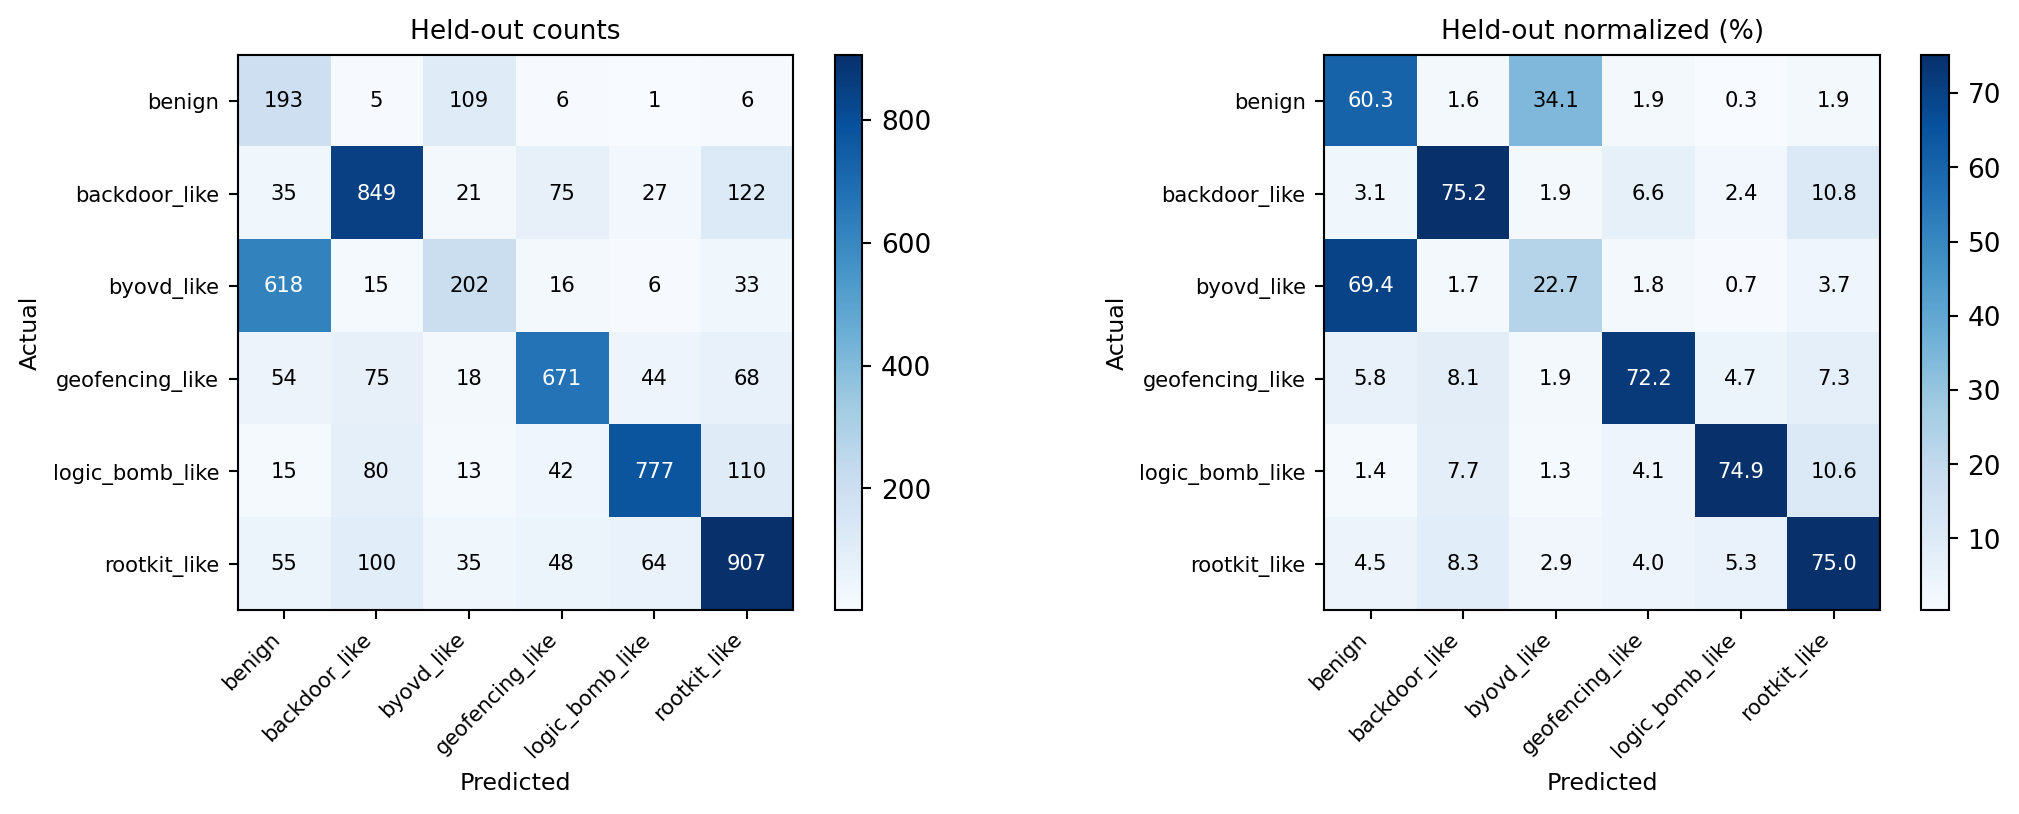
\includegraphics[width=0.74\textwidth]{figs/holdout_confusion.png}
    \caption{ماتریس درهم‌ریختگی بهترین مدل چرخه سوم (\lr{ResNet50} روی \lr{S3}) روی \num{۵٬۵۱۵} نمونه نگه‌داشته‌شده. سطر \lr{byovd\_like} الگوی غالب سردرگمی با کلاس \lr{benign} را نشان می‌دهد.}
    \label{fig:cm}
\end{figure}

\subsection{چرخه چهارم: مدول ادغام هرمی و فیلتر‌های بافت}
چرخه چهارم به دو کاستی دیگر می‌پردازد. مقاله در نتیجه‌گیری پیشنهاد می‌کند که با سازوکار توجه بتوان نواحی مهم تصویر را برجسته کرد ولی آن را پیاده نمی‌کند؛ ما یک سر ادغام هرمی\pn{Pyramid Pooling Module (PPM)} با الهام از \lr{PSPNet} \cite{zhao2017pspnet} و چهار مقیاس $1\times1$ تا $6\times6$ را به‌عنوان نزدیک‌ترین گام عملی به آن ایده آزمودیم. همچنین مقاله بایت‌ها را تنها به‌عنوان شدت روشنایی خام می‌دهد و از توصیفگر‌های بافت صریح استفاده نمی‌کند؛ ما دو کانال بافتی افزودیم که در زمان اجرا محاسبه می‌شوند: الگوی دودویی محلی\pn{Local Binary Pattern (LBP)} \cite{ojala2002lbp} و پاسخ یک فیلتر گابور. در مجموع ۲۶ پیکربندی زیر توصیف \kd{arm\_zephyr\_optimized\_ppm} اجرا شد.

نتیجه یک شکست کامل بود. بهترین پیکربندی این چرخه تنها به \pct{۲۴٫۸۶} رسید و پیکربندی \lr{ResNet50} روی \lr{S3} که در چرخه سوم \pct{۶۵٫۲۶} داشت، با افزودن \lr{PPM} به \pct{۱۴٫۲۹} سقوط کرد. میانگین افت روی ۱۹ پیکربندی مشترک میان دو چرخه برابر \num{۲۰٫۷} واحد است. شکل \ref{fig:ppm} منحنی‌های آموزش را کنار هم می‌گذارد و نکته تعیین‌کننده را آشکار می‌کند: با \lr{PPM}، صحت \emph{مجموعه آموزش} نیز از \pct{۲۵} فراتر نمی‌رود. یعنی این یک شکست در تعمیم نیست، بلکه شکست در برازش است.

\begin{figure}[!ht]
    \centering
    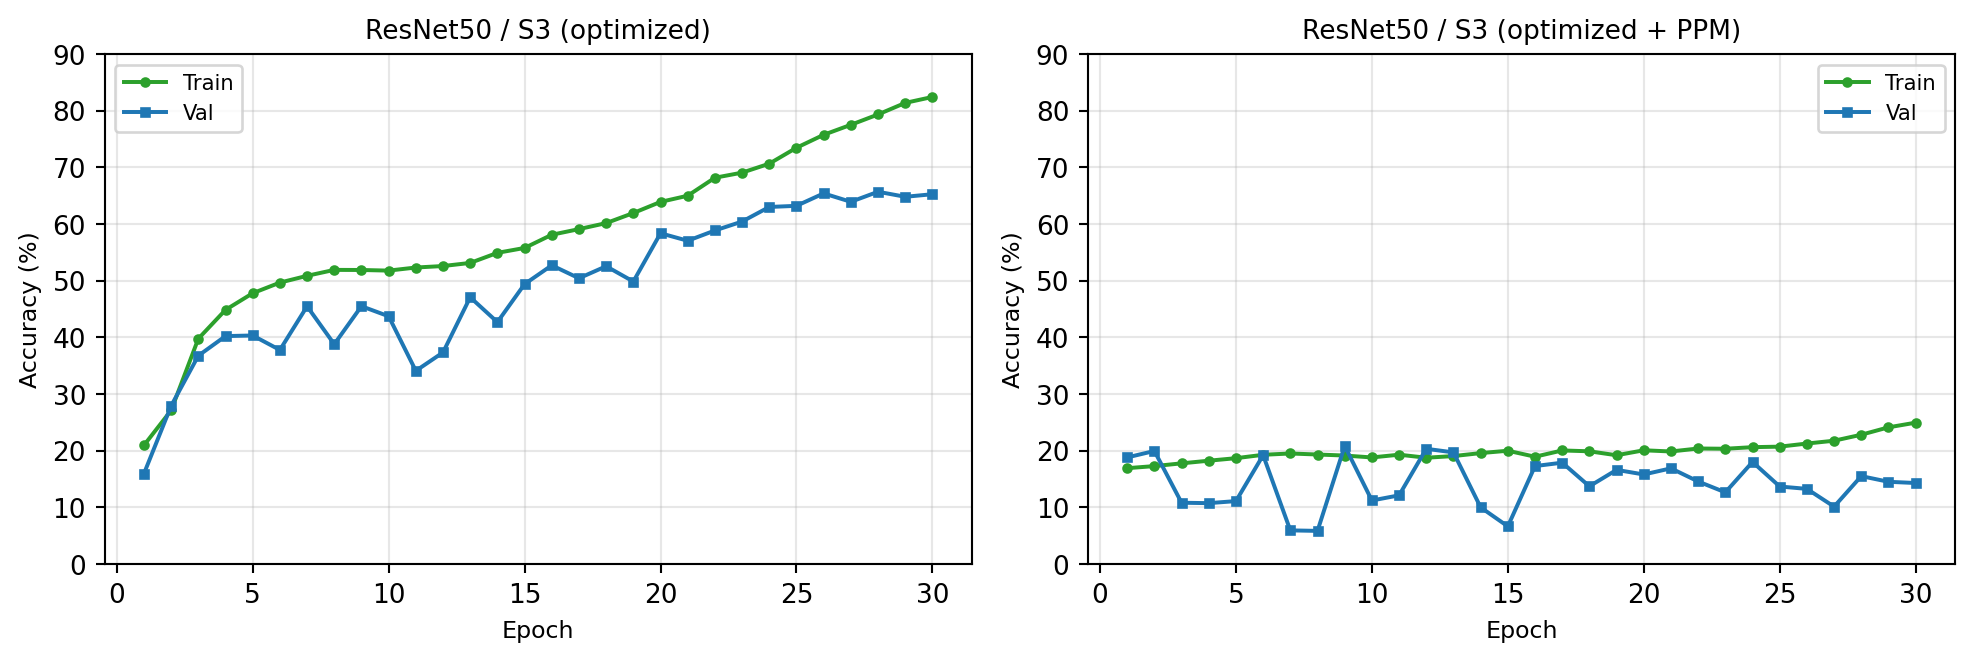
\includegraphics[width=0.82\textwidth]{figs/ppm_curves.png}
    \caption{منحنی‌های آموزش \lr{ResNet50} روی \lr{S3}، با و بدون سر ادغام هرمی. در نمودار راست، صحت آموزش نیز در سطح تصادفی می‌ماند؛ نشانه شکست بهینه‌سازی و نه بیش‌برازش.}
    \label{fig:ppm}
\end{figure}

\paragraph{ریشه‌یابی.} بازخوانی کد سه علت مشخص را نشان می‌دهد و هر سه به پیاده‌سازی ما برمی‌گردند، نه به ایده \lr{PPM}:
\begin{enumerate}[leftmargin=1.6em,itemsep=0.1em,topsep=0.2em]
    \item هر شاخه هرم پس از ادغام به اندازه $s \times s$ و یک پیچش $1\times1$، دوباره یک \kd{AdaptiveAvgPool2d(1)} می‌خورد؛ یعنی همان اطلاعات مکانی چندمقیاسی که کل هدف \lr{PPM} است بی‌درنگ میانگین‌گیری و دور ریخته می‌شود، در حالی که در \lr{PSPNet} اصلی نقشه‌های ادغام‌شده بازنمونه‌برداری و به‌صورت \emph{مکانی} الحاق می‌شوند. آنچه ساختیم یک هرم نیست، بلکه چهار توصیفگر سراسری تقریباً زائد است.
    \item این سر برای \lr{ResNet50} حدود \num{۴٬۱۹۴٬۳۰۴} پارامتر پیچشی با مقداردهی تصادفی می‌افزاید که با نرخ یادگیری \num{۰٫۰۱} و کاهش وزن \num{۰٫۰۰۶} جدول \ref{tab:hyper} آموزش می‌بیند؛ گرادیان‌های اولیه آن، ویژگی‌های از پیش‌آموخته ستون فقرات را در همان دوره‌های نخست تخریب می‌کنند.
    \item در \lr{VGG16} جایگزینی \kd{avgpool} با این سر، ورودی \kd{classifier[0]} را از \num{۲۵٬۰۸۸} به \num{۱٬۰۲۴} می‌کاهد و وزن‌های از پیش‌آموخته آن لایه نیز دور ریخته می‌شوند.
\end{enumerate}
پس نتیجه‌گیری درست آن است که \textbf{پیاده‌سازی ما از \lr{PPM} نادرست بوده}، نه اینکه ادغام هرمی برای این مسئله نامناسب است؛ توضیحی از جنس «شکستن ناوردایی انتقالی» هم سازگار نیست، چون چنین استدلالی درباره تعمیم است و اینجا مدل حتی داده آموزش را برازش نمی‌کند. کانال‌های \lr{LBP} و گابور نیز زیر سایه همین شکست اجرا شدند و درباره سودمندی مستقل آن‌ها نمی‌توان نتیجه‌ای گرفت؛ ضمن اینکه فیلتر گابور پیاده‌شده تنها یک جهت و یک بسامد دارد، در حالی که کاربرد متعارف آن یک بانک چندجهته است.

\subsection{هزینه محاسباتی و نقش موازی‌سازی}
مجموع زمان آموزش چهار چرخه حدود \num{۸۷} ساعت پردازنده گرافیکی است (به‌ترتیب \num{۱۵٫۴}، \num{۱۴٫۳}، \num{۲۵٫۲} و \num{۳۱٫۶} ساعت) و همه اجرا‌ها روی نمونه‌های رایگان کگل انجام شدند. این عدد به‌تنهایی گمراه‌کننده است، چون سقف زمان هر جلسه کگل محدود است و اجرای سریالی چنین حجمی عملاً ناممکن بود. راهکار ما تقسیم متوازن پیکربندی‌های هر چرخه میان سه تا چهار نمونه موازی بود؛ با این تقسیم، زمان دیواری هر چرخه به‌طور میانگین به حدود ۳ ساعت برای دو چرخه نخست، ۶ ساعت برای چرخه سوم و ۱۰ ساعت برای چرخه چهارم رسید. بدون این موازی‌سازی، آزمودن ۸۵ پیکربندی در بازه این فاز ممکن نبود و ناچار می‌شدیم مطالعه حذفی را به چند پیکربندی محدود کنیم؛ یعنی دقیقاً همان کمبودی که در \S\ref{sec:critique} به مقاله گرفتیم. ضمناً چرخه چهارم با میانگین ۱۰ ساعت به سقف زمان جلسه نزدیک شده بود و فضای بیشتری برای گسترش نمی‌گذاشت.
